\section{Intepretation}
\label{sec:Interpretation}

In general, the bright and hard gamma-ray emission at the base of the bubbles can be at any position along the line of sight.
In this section we consider two characteristic scenarios: that the emission is near the GC at the base of the FB and that the emission is 
produced by one or a few SNe closer to us (similar to, e.g., Cygnus region that contains recently accelerated CR from several SNe).

\subsection{Emission near the GC scenario}

In the estimates in this subsection we will use the following characteristic sizes: 
the distance to the GC is $\SI{8.5}{kpc}$, 
the size of the region with the enhanced gamma-ray emission interpreted as an additional population of CR:
$-10^\circ < \ell < 0^\circ$ and $|b| < 6^\circ$.
If we assume that the geometry of the region is a simple box, then the size of the box along the GP is $\SI{1.5}{kpc}$,
while the half-size in the vertical direction (distance from the GP to the boundary) is $\Delta h = 0.9$ kpc.
%\red{Dima: for the total CR energy content, we should use the $|b| < 6^\circ$ ROI.}

One of the most intriguing features of the gamma-ray spectrum at the base of the FB is the absence of the cutoff up to 1 TeV and 
a hard spectrum of underlying electrons or protons.
In particular, the spectrum of the CRp is $\sim E^{-2.2}$ which is significantly harder than the propagated spectrum
$\sim E^{-2.7}$ observed locally and throughout most of the GP.
We will assume that the CRp spectrum at the base of the bubbles is equal to the injection spectrum unaffected by the 
propagation softening.
This is possible if the CRp were injected relatively recently and didn't have time to escape from the region of the enhanced emission,
i.e., the age of the CRp is smaller than the propagation time to cross the vertical distance of 0.9 kpc.

We will assume a spatially constant diffusion coefficient $D(E) = D_0\left(\frac{E}{\SI{1}{GeV}}\right)^\delta$ with $D_0 = \SI{3e28}{cm^2/s} = \SI{100}{pc^2/kyr}$ and $\delta = 0.4$.
The escape time for the protons (and also electrons) at $E = \SI{10}{TeV}$ is 
\Laura{Should we also use 3 TeV here? Then escape time is 165 kyr.} 
\dima{it looks from Table 2 that the cutoff for the protons within $2^\circ$ from the Gal plane is 20 TeV? 
Strictly speaking, we should use 20 TeV for the protons (and 3 TeV for the electrons).} 
\be
T_{\rm esc} = \frac{\Delta h^2}{2 D(E)} \approx \SI{100}{kyr}.
\ee
%\Laura{Is there no factor of 1/2 missing in the formula for the cooling time?} \dima{good point - fixed.}
This gives us an approximate upper bound on the age of the proton CR.
The CRp energy density (normalized to $n_\Hy = \SI{1}{cm^{-3}}$) within $|b| < 2^\circ$ is 
$\de E_\tot / \de V = \SI{360}{meV\: cm^{-3}}$ between $\SI{1}{GeV}$ and $\SI{1}{TeV}$.
In Figure \ref{fig:Particle_spectra} (left), we compare the corresponding flux to the local CRp flux.
The total energy content within $|b| < 6^\circ$ is $E_\tot = \SI{7e52}{erg}$.
%However, the gas density in the inner Galaxy is probably higher than $n_\Hy = \SI{1}{/cm^3}$ as assumed in Section \ref{sec:Pion_model}, resulting in an energy content in protons of the same order of magnitude as the energy density in electrons.
This population of CRp can be obtained from $\sim$ 700 SNe in the past $\sim \SI{100}{kyr}$, 
assuming that on average SNe inject $\sim 10^{50}$ erg in CRp (which corresponds to about 10\% efficiency).
%\Laura{Why 500 kyr? } \dima{ sorry this was a typo from my previous estimates.}\\
\\


The best-fit spectrum of CR electrons is $\sim E^{-2.7}$ which is softer than the spectrum of the protons.
Nonetheless, this spectrum is harder than the spectrum expected in the presence of cooling softening
for a stationary population of CRe or a break for a transient population of CRe.
Thus, unless the injection spectrum is harder than $E^{-2}$, the population of the CRe at the base of the 
bubbles is not affected by cooling up to $\SI{3}{TeV}$,
which is the 95\% confidence minimal lower bound on the cutoff in the CRe. 
The cooling time for the electrons at %$\SI{100}{TeV}$ cooling to 
$\SI{3}{TeV}$ is $T_{\rm cool} \approx \SI{180}{kyr}$,
%\Laura{I integrated from 100 TeV to 3 TeV.} The distance that the electrons at $\SI{3}{TeV}$ propagate during $\SI{180}{kyr}$ is $\SI{0.85}{kpc}$ 
%\Laura{Can I just say 180 kyr $\approx$ 200 kyr.} \dima{ OK, this is also similar to the escape time at 3 TeV.}, 
%this corresponds to \red{$xx^\circ$ -- this is consistent(?) with the 
%softening of CRe for $|b| > 2^\circ$}.
which is comparable to the escape time at $\SI{3}{TeV}$.

The total energy density in electrons with energy above $E_0 = \SI{1}{GeV}$, which needs to be generated by this transient process, is given by the integral of the electron spectrum that was found in Section \ref{sec:IC_model}:
\be
\frac{\de E_\tot}{\de V} = \int_{E_0}^{\infty} \left(E \frac{\de N}{\de E}\right)_{\!\!\el} \de E = \SI{4.0}{meV/cm^3}.
\ee
In Figure \ref{fig:Particle_spectra} (right), we compare the corresponding flux to the local CRe flux.
The total energy content of the ROI in electrons above $\SI{1}{GeV}$ is $E_\tot = \SI{3e51}{erg}$, which corresponds to the CR energy output of 3000 SNe in the past $\approx \SI{200}{kyr}$ assuming a 0.1\% efficiency in converting the SNe kinetic energy to CRe energy.
The ratio of the electron to proton acceleration efficiencies $K_{ep} = 10^{-2}$ assumed here is likely too optimistic,
given that the typical values of the ratio of efficiencies are $\sim 10^{-3}$.
Since the escape time is comparable to the electron cooling time and the required number of SNe in the hadronic
scenario is smaller than the number of SNe in the leptonic scenario (for the ratio of acceleration efficiencies $K_{ep} \lesssim 10^{-2}$),
we conclude that the majority of the gamma-ray emission near the base of the FB 
is likely to be produced by the hadronic interactions of CRp with the gas.
%\Laura{So, $\SI{1e50}{erg}$ per SN?} \dima{ SNe kinetic energy is $10^{51}$ erg, energy in CRs:  $10^{50}$ erg, a fraction of that is in CRe, i.e., if we have 1\% in electrons, then we need 300 SNe.}
%\dima{if the electrons cool as they propagate $2^\circ$, we should use $|b| < 2^\circ$ to calculate the total energy content of CRe}. \Laura{This is the total energy content for $|b| < 6$} \dima{OK}.
\begin{comment}
We note, that the energy density of CRe is comparable to the energy density of CRp 
(especially if we take the density of gas $n_\Hy = \SI{10}{cm^{-3}}$).
Since we expect that in SN explosions CRp are accelerated at the same rate or better than CRe,
there should be a significant hadronic component of the gamma-ray emission.
The presence of the leptonic component, on the other hand, is not necessary.
Since the escape time at $\SI{10}{TeV}$ is much longer than the electron cooling time at 10 TeV, \Laura{The escape time is comparable to the cooling time.}
the less efficient acceleration of CRe in SNe and cooling may lead to subdominant contribution of 
IC scattering at $E_\g = 1$ TeV relative to the hadronic model of the gamma-ray production.
\end{comment}
The presence of the hadronic production of gamma-rays at the base of the FB without a sign of a cutoff up to gamma-ray energies
of 1 TeV is important for the detectability of the associated neutrino signal by the neutrino telescopes.

\begin{figure*}[h]
    \begin{subfigure}{0.5\textwidth}
        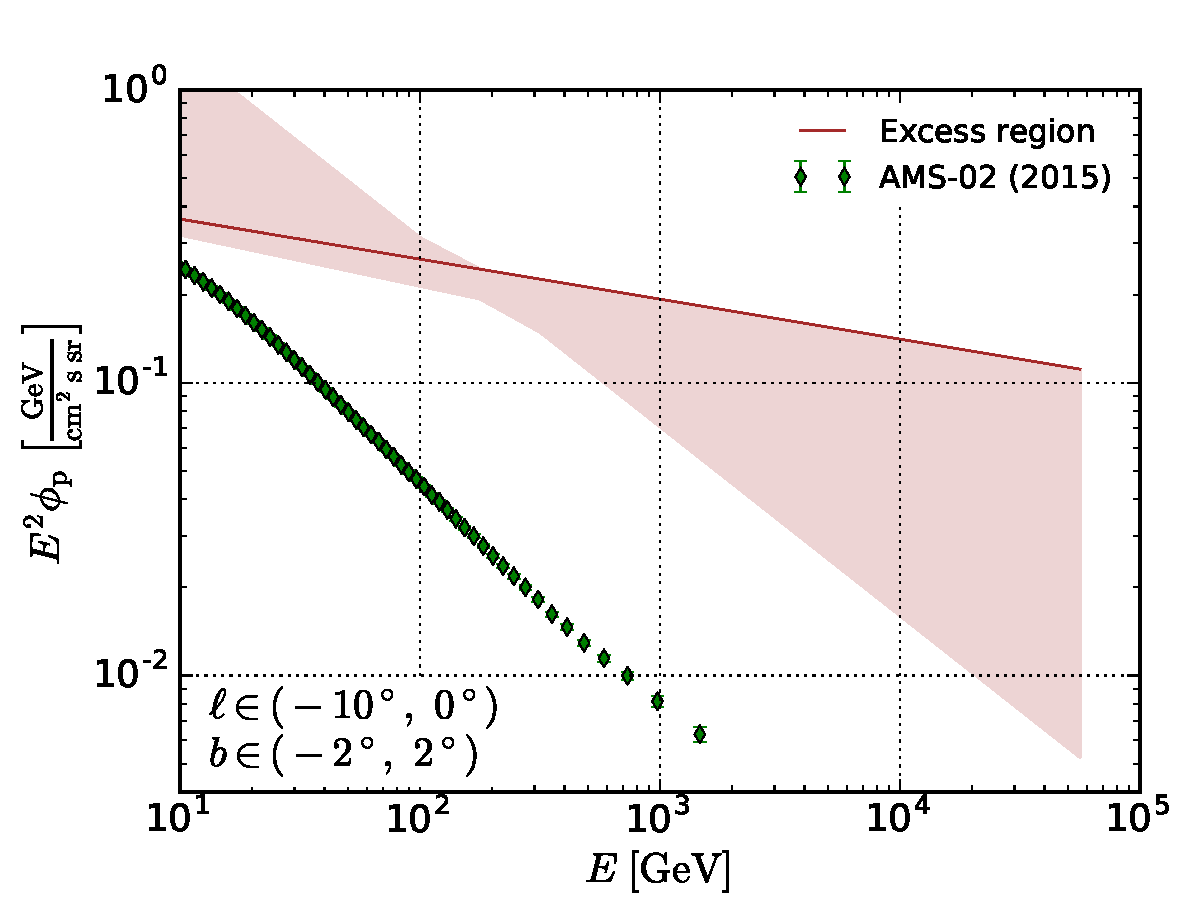
\includegraphics[width=\textwidth]{plots/Summary_proton_spectra_0.pdf}
    \end{subfigure} 
    \begin{subfigure}{0.5\textwidth}
        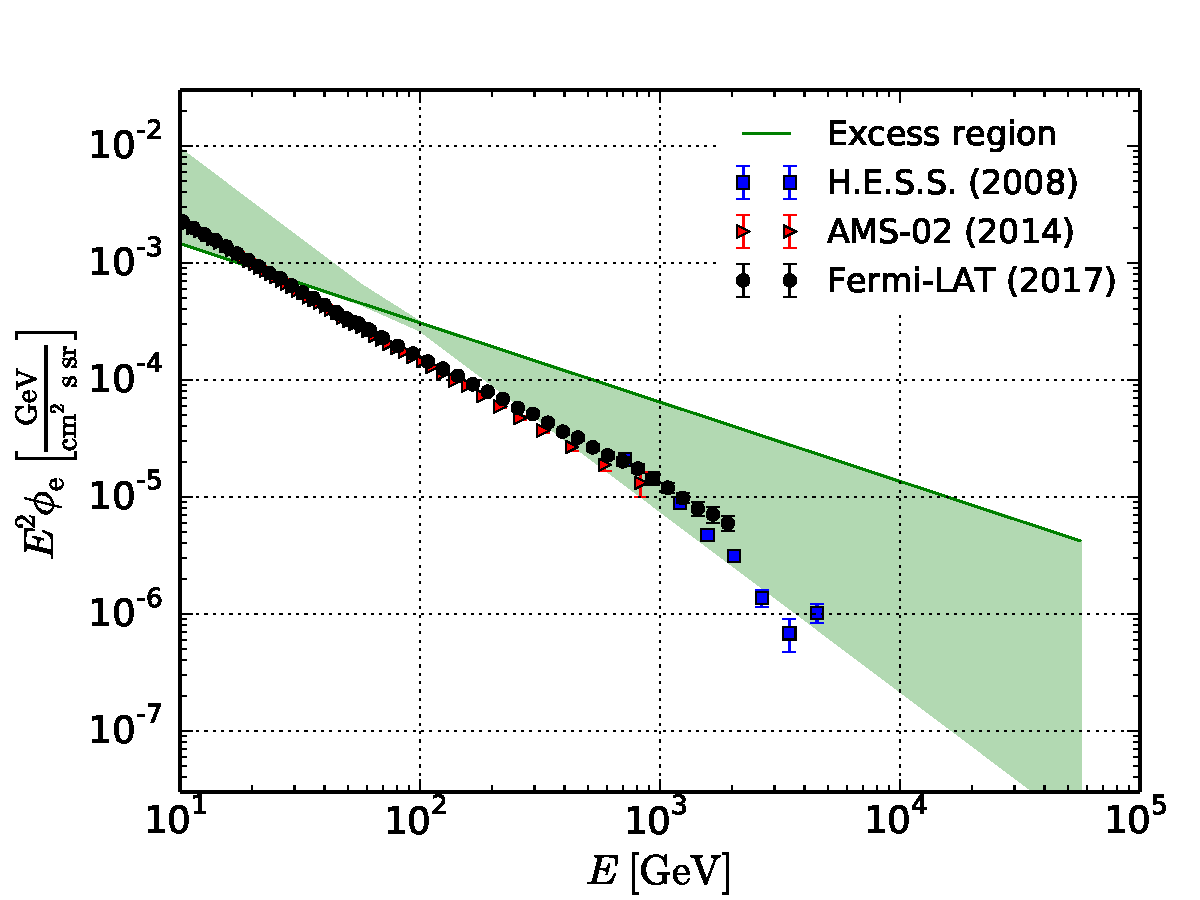
\includegraphics[width=\textwidth]{plots/Summary_electron_spectra_0.pdf}
    \end{subfigure}
  	\caption{Best-fit proton (left) and electron (right) spectra for the baseline model. The shaded bands represent the systematic uncertainties, estimated by the maximal and minimal best-fit spectrum of the other models. For comparison with the local CR spectrum, data points of some experiments are shown. The errorbars represent the systematic + statistical errors estimated in the references.}
  	\label{fig:Particle_spectra}
\end{figure*}


\section{Conclusions}